\def\CC{{C\nolinebreak[4]\hspace{-.05em}\raisebox{.4ex}{\tiny\bf ++}}}
%
\begin{frame}\frametitle{ESDG in \mirgecom{}}
\vspace{15pt}
\begin{center}
\mirgecom{} ESDG branch: https://github.com/illinois-ceesd/mirgecom@production-esdg
\end{center}
%\begin{multicols}{2}
\begin{itemize}
\item Implmentation status
\begin{itemize}
\item Work of Thomas Gibson modernized (grudge, mirgecom)
\item CNS and Euler w/ ESDG for inviscid terms
\end{itemize}
\item Using ESDG in \mirgecom{}
\begin{itemize}
\item Driver update
\item Examples
\end{itemize}
%\end{itemize}
\item Troubles
\begin{itemize}
\item Multicomponent diffusion (advection ok)
\item Prediction boundary issue
\end{itemize}
\item Can be improved...
\end{itemize}
%\columnbreak
%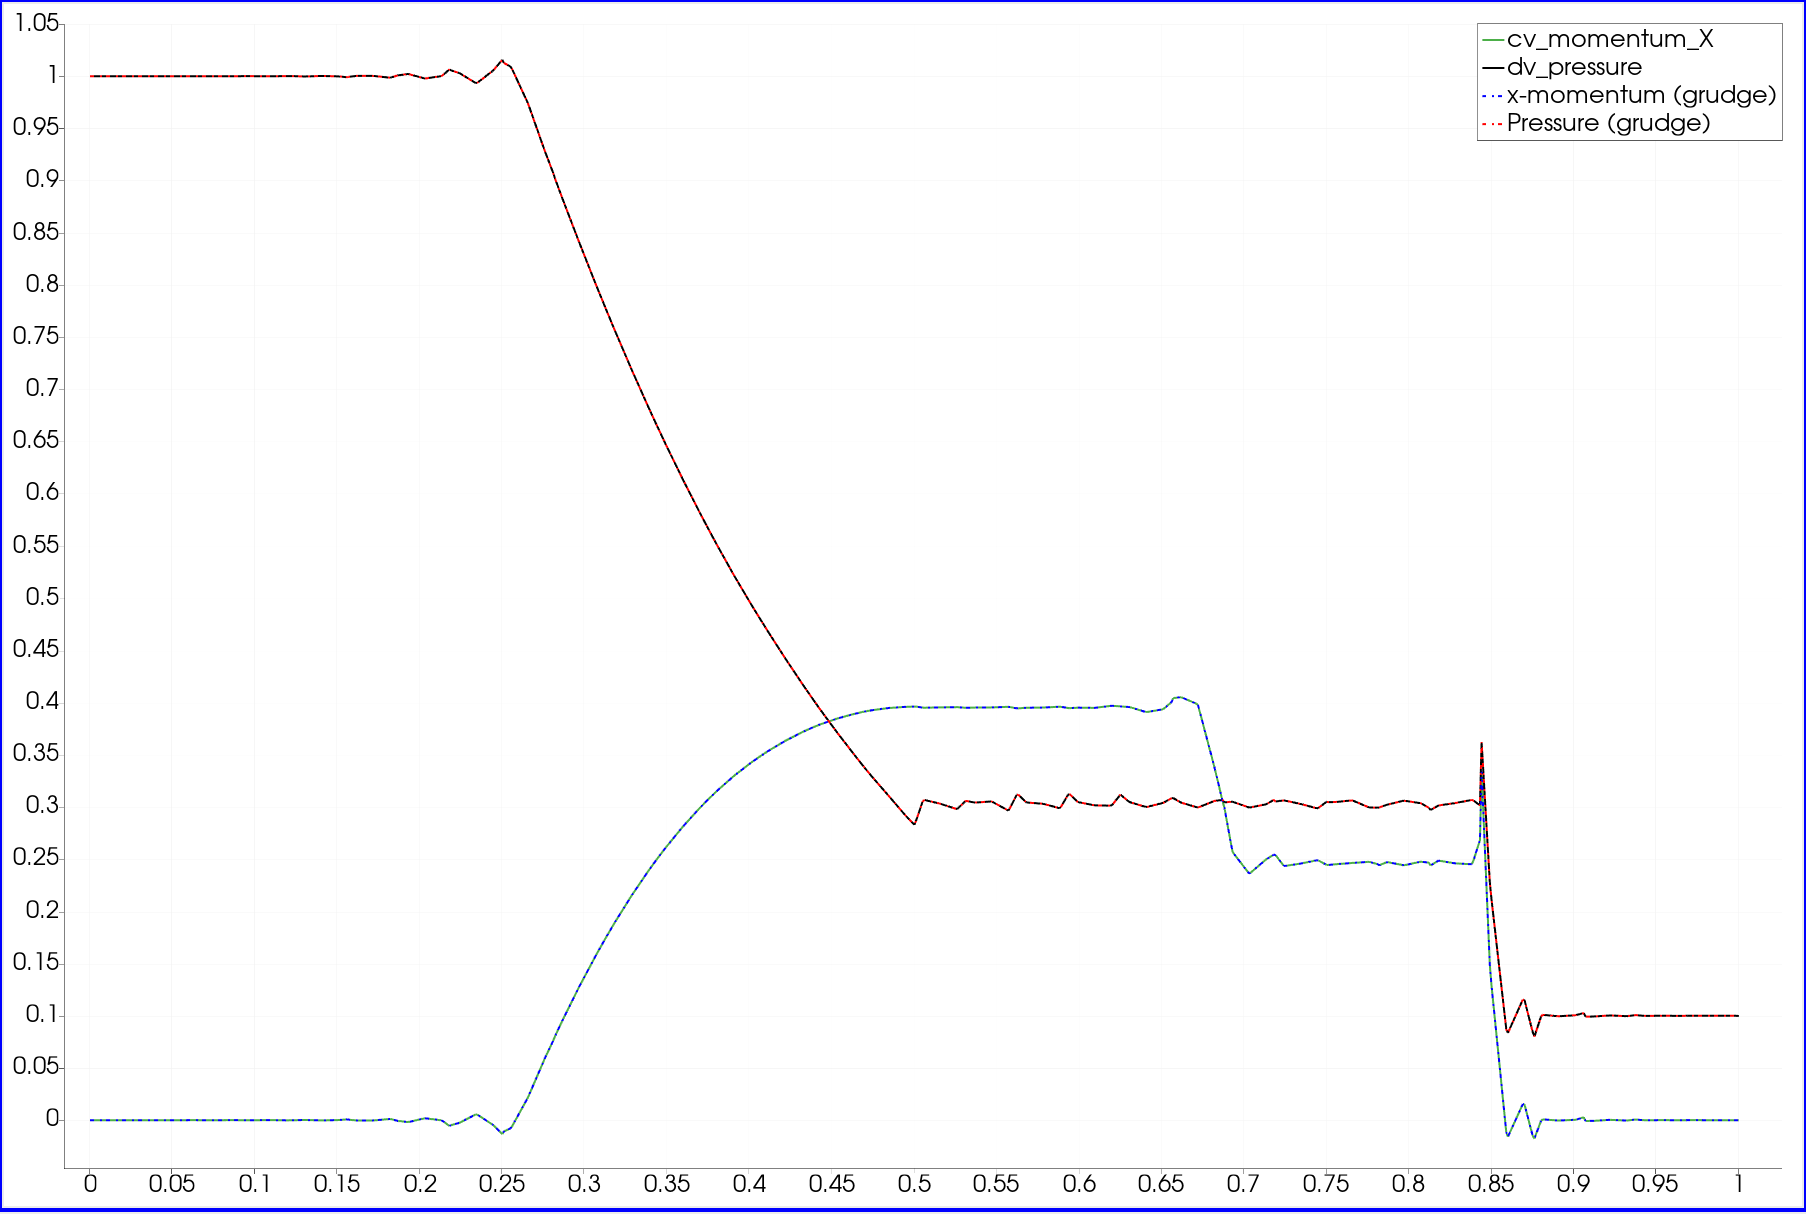
\includegraphics[width=.48\textwidth]{figures/compare-sod-shock-esdg-grudge.png}
%\end{multicols}
\end{frame}

\begin{frame}[fragile]\frametitle{ESDG Procedure in \mirgecom{}}
\begin{multicols}{2}
\begin{itemize}
\setlength{\itemsep}{3pt}
\item Project fluid conserved variables ($CV$) to quadrature points
\item Calculate Entropy Variables ($EV$) from projected $CV_q$
\item Project $EV$ to element boundaries (communicate too)
\item Compute modified $CV$, (${CV}^\prime$) from projected $EV$
\item Flux ${CV}^\prime$ using
\begin{itemize}
\item usual $CV$ BCs and
\item entropy-conserving flux routines
\end{itemize}
\item Hit with DG div operator for RHS
\end{itemize}
\columnbreak
\begin{center}
entropy\_stable\_euler\_operator
\end{center}
\vspace{-10pt}
\begin{lstlisting}
# Interpolate state to vol quad grid
cv_q = project_fluid_state(vol, quad, state)

# Compute the projected (nodal) entropy variables
ev = volume_quadrature_project(
      quad,
      # Map to entropy variables
      conservative_to_entropy_vars(gamma, cv_q)
     )

# Makes [vol, surf] two-point flux-ready array
cv_prime = \
  make_entropy_projected_fluid_state(
     vol, faces, cv, ev)

# EC volume flux for CV'
flux_matrices = \
   entropy_conserving_flux_chandrashekar(
      gas_model, cv_prime))

# Compute volume derivatives using flux differencing
vol_term = \
  -volume_flux_differencing(quad, faces_quad,
                            flux_matrices)

# CV' on interior faces
cv_mod_interior_pairs = [
  _interp_modified_cv(gamma, tpair)
  for tpair in interior_trace_pairs(dcoll, ev)
]

# CV' on domain bnd
domain_bnd_states = {
  btag: project_fluid_state(
    dcoll, dd_vol,
    as_dofdesc(btag).with_discr_tag(quadrature_tag),
    cv, entropy_stable=True)
    for btag in boundaries
}

# Compute interface contributions
flux_bnd = \
  inviscid_flux_on_element_boundary(
    dcoll, gas_model, boundaries, cv,
    domain_bnd_states)

# RHS = div(ec-fluxes) 
return div_operator(vol_term, flux_bnd)

\end{lstlisting}
\end{multicols}
% Note: uses native mirgecom boundaries, but with CV' and EC fluxes
\end{frame}

\begin{frame}\frametitle{Using ESDG in \mirgecom{}}
\begin{multicols}{2}
\begin{itemize}
\item Install \mirgecom{} ESDG branch
\item Update your driver
\begin{itemize}
\item ESDG is lazy-only
\item Use Overintegration (default order$=2p+1$)
\item Use ESDG operators
\end{itemize}
\item Examples:
\begin{itemize}
\item sod-mpi.py
\item pulse-mpi.py
\item vortex-mpi.py
\item taylor-green-mpi.py
\item poieuille-mpi.py
\item combozzle-mpi.py
\item thermally-coupled-mpi.py
\end{itemize}
\end{itemize}
% include some performance numbas
\columnbreak
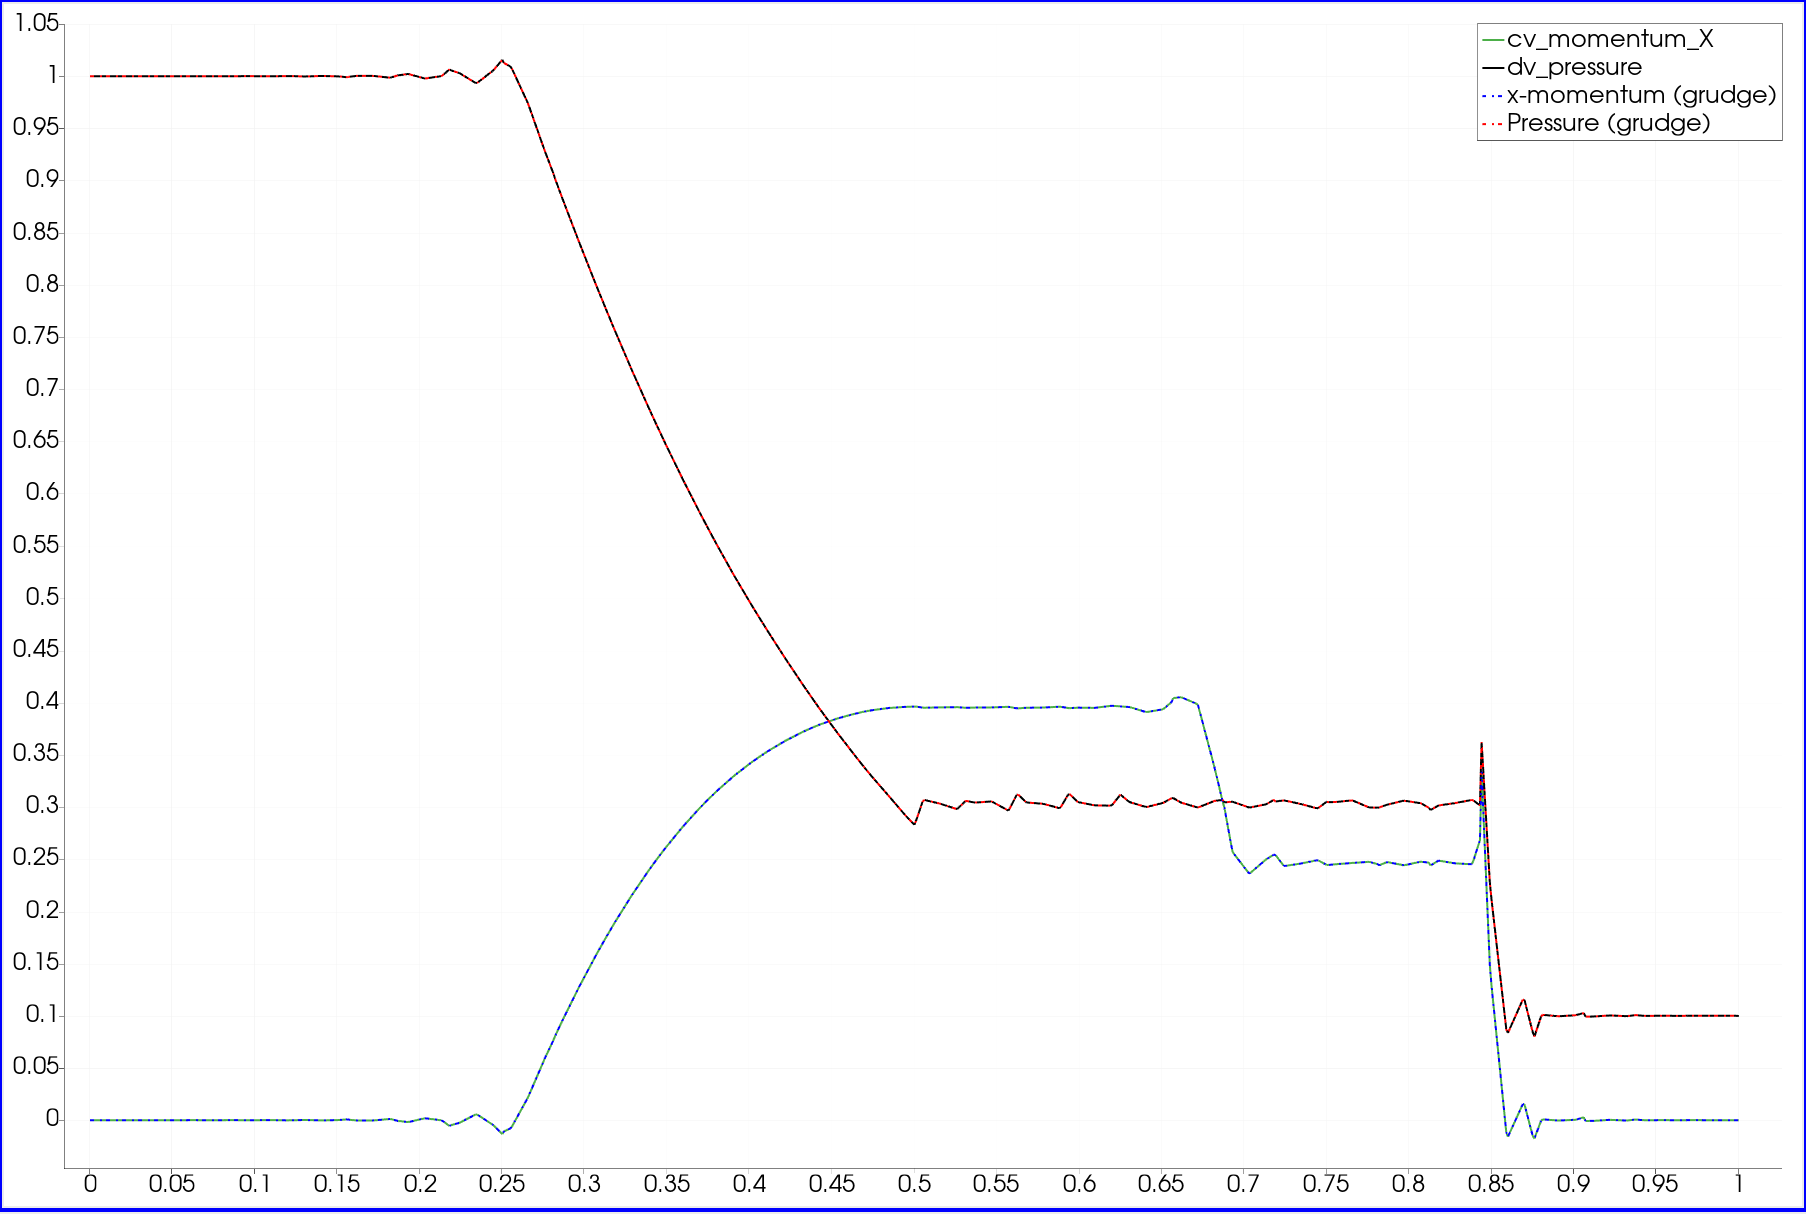
\includegraphics[width=.48\textwidth]{figures/compare-sod-shock-esdg-grudge.png}
\end{multicols}
\end{frame}

\begin{frame}\frametitle{ESDG Status for Prediction}
\begin{multicols}{2}
\begin{itemize}
\item ESDG-enabled prediction
\begin{itemize}
\item \mirgecom{} PR\#877
\item \textit{drivers\_y3-prediction} PR\#26
\end{itemize}
\item Currently making nans near the isothermal noslip boundaries
\item Debugging
\begin{itemize}
   \item Runs multiphysics example without issue
   \item Running Poiseuille isothermal noslips without issue 
   \item Will use Shock1D to debug more
\end{itemize}
\end{itemize}
\columnbreak
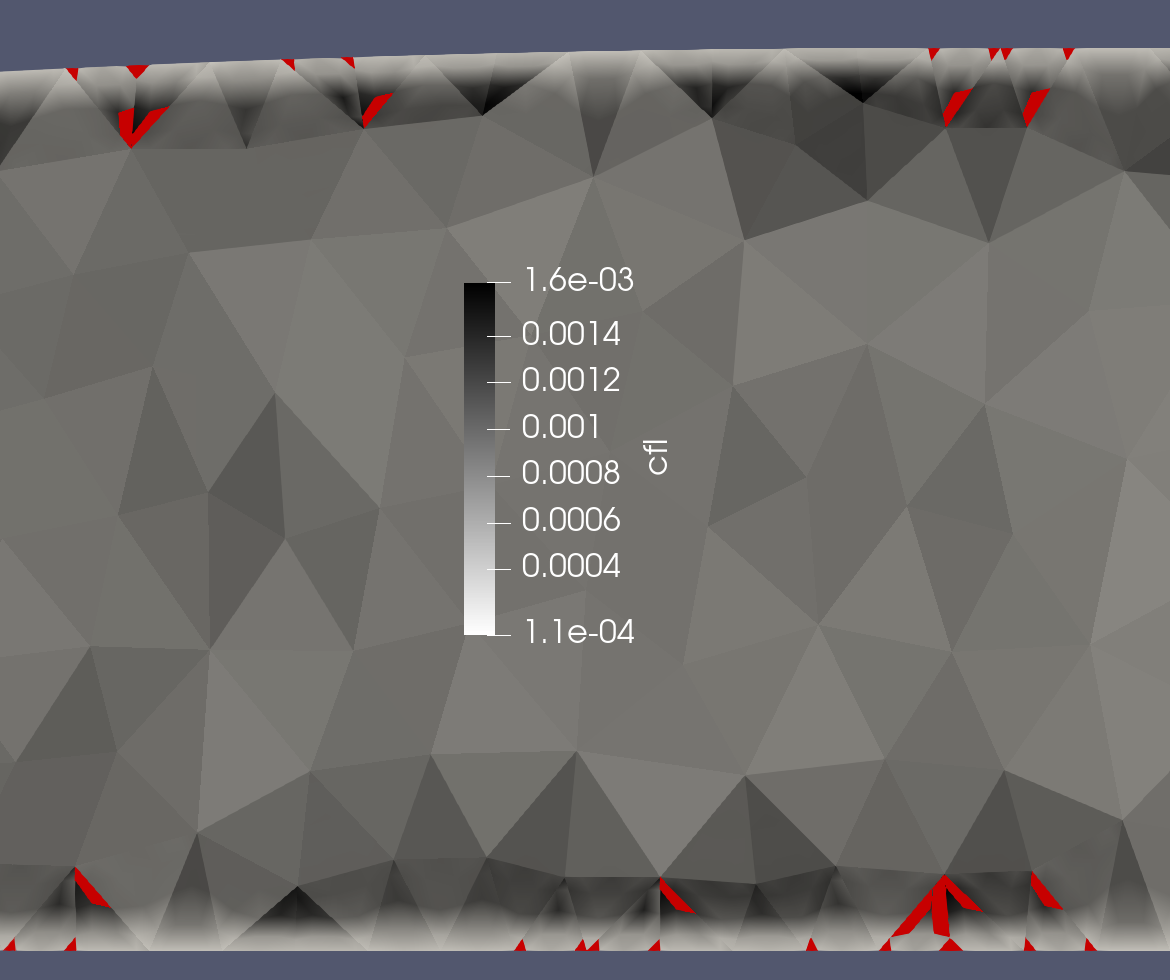
\includegraphics[width=.48\textwidth]{figures/prediction-esdg-nans.png}
\end{multicols}
\end{frame}

\begin{frame}\frametitle{What's next for ESDG?}
\begin{itemize}
\item Prediction w/ESDG is then main priority, then ...
\item Eliminate the glued-together vol/surf construction in grudge
\item Better integration with the native operators
\item Fix bugs in multi-component, and mixtures cases
\item Extend to viscous terms
\end{itemize}
\end{frame}
